\documentclass{article}
\usepackage[top=1in, bottom=1in, left=1in, right=1in]{geometry}
\usepackage{graphicx}
\begin{document}

\begin{flushright}
Matt Jibson \\
EG510 \\
HW 8
\end{flushright}

Problems solved using LINDO. \\

\textbf{Production Planning (tomatoes):}

\begin{verbatim}
MAX = 0.082 * AW + 0.082 * BW + 0.066 * AJ + 0.066 * BJ + 0.074 * AP + 0.074 * BP;
AW - 3 * BW > 0;
3 * AJ - BJ > 0;
AW + BW < 14400000;
AJ + BJ < 1000000;
AP + BP < 2000000;
AW + AJ + AP < 600000;
BW + BJ + BP < 2400000;
\end{verbatim}

Results:

\begin{verbatim}
Global optimal solution found.
Objective value:                              225200.0
Total solver iterations:                             5

                       Variable           Value        Reduced Cost
                             AW        525000.0            0.000000
                             BW        175000.0            0.000000
                             AJ        75000.00            0.000000
                             BJ        225000.0            0.000000
                             AP        0.000000           0.3200000E-01
                             BP        2000000.            0.000000

                            Row    Slack or Surplus      Dual Price
                              1        225200.0            1.000000
                              2        0.000000          -0.8000000E-02
                              3        0.000000          -0.8000000E-02
                              4       0.1370000E+08        0.000000
                              5        700000.0            0.000000
                              6        0.000000           0.1600000E-01
                              7        0.000000           0.9000000E-01
                              8        0.000000           0.5800000E-01
\end{verbatim}

1. Red Brand Canners should produce $525,000 + 175,000 = 700000 / 18 = 38,887$ cases of canned whole, $75,000 + 225,000 = 300000 / 20 = 15,000$ cases of tomato juice, and $2,000,000$ cases of tomato paste. Net profit is $1.48 * 38887 + 1.32 * 15000 + 1.85 * 2,000,000 = \$3,777,352.76$. \\

2. Since dual price for row 7 is \$0.09, we determine that it is profitable for them to buy at least some of the additional Grade A lot. The sensitivity output:

\begin{verbatim}
Ranges in which the basis is unchanged:

                                      Objective Coefficient Ranges
                                  Current        Allowable        Allowable
                Variable      Coefficient         Increase         Decrease
                      AW    0.8200000E-01        0.1546667    0.2133333E-01
                      BW    0.8200000E-01        0.4640000    0.2133333E-01
                      AJ    0.6600000E-01    0.2133333E-01        0.1546667
                      BJ    0.6600000E-01    0.1422222E-01    0.5155556E-01
                      AP    0.7400000E-01    0.3200000E-01         INFINITY
                      BP    0.7400000E-01         INFINITY    0.1600000E-01

                                           Righthand Side Ranges
                     Row          Current        Allowable        Allowable
                                      RHS         Increase         Decrease
                       2              0.0         466666.7         600000.0
                       3              0.0         1400000.         200000.0
                       4    0.1440000E+08         INFINITY    0.1370000E+08
                       5         1000000.         INFINITY         700000.0
                       6         2000000.         200000.0         466666.7
                       7         600000.0         600000.0         466666.7
                       8         2400000.         466666.7         200000.0
\end{verbatim}

From this we see that it is profitable for up to 600,000 lbs of Grade A tomatoes, so we recommend that they buy the entire lot of 80,000. \\

\textbf{Dynamics of Toy Train:}

\begin{verbatim}
MIN = y + 0.01 * z;

x1_1 - 1 > -y;
x1_1 - 1 < y;
u_2 - u_1 > -z;
u_2 - u_1 < z;

x1_2 - 2 > -y;
x1_2 - 2 < y;
u_3 - u_2 > -z;
u_3 - u_2 < z;

x1_3 - 3 > -y;
x1_3 - 3 < y;
u_4 - u_3 > -z;
u_4 - u_3 < z;

x1_4 - 4 > -y;
x1_4 - 4 < y;
u_5 - u_4 > -z;
u_5 - u_4 < z;

x1_1 = 0.048374 * u_1;
x1_2 = x1_1 + 0.95163 * x2_1 + 0.048374 * u_2;
x1_3 = x1_2 + 0.95163 * x2_2 + 0.048374 * u_3;
x1_4 = x1_3 + 0.95163 * x2_3 + 0.048374 * u_4;
x1_5 = 5;

x2_1 = 0.95163 * u_1;
x2_2 = 0.90484 * x2_1 + 0.95163 * u_2;
x2_3 = 0.90484 * x2_2 + 0.95163 * u_3;
x2_4 = 0.90484 * x2_3 + 0.95163 * u_4;
x2_5 = 0;

@FREE(u_1);
@FREE(u_2);
@FREE(u_3);
@FREE(u_4);
@FREE(u_5);
\end{verbatim}

Results for $c = 0.01$:

\begin{verbatim}
Objective value:                             0.8983354

                       Variable           Value        Reduced Cost
                              Y       0.8514394            0.000000
                              Z        4.689601            0.000000
                           X1_1       0.1485606            0.000000
                            U_2       -1.618517            0.000000
                            U_1        3.071084            0.000000
                           X1_2        2.851439            0.000000
                            U_3       -1.049907            0.000000
                           X1_3        3.851439            0.000000
                            U_4        0.000000            0.000000
                           X1_4        3.851439            0.000000
                            U_5        4.689601            0.000000
                           X2_1        2.922536            0.000000
                           X2_2        1.104198            0.000000
                           X2_3        0.000000           0.5025365E-03
                           X1_5        5.000000            0.000000
                           X2_4        0.000000            0.000000
                           X2_5        0.000000            0.000000
\end{verbatim}

Results for $c = 0.1$:

\begin{verbatim}
Objective value:                             0.9656577

                       Variable           Value        Reduced Cost
                              Y       0.9488806            0.000000
                              Z       0.1677710            0.000000
                           X1_1       0.5111943E-01        0.000000
                            U_2       0.8889833            0.000000
                            U_1        1.056754            0.000000
                           X1_2        1.051119            0.000000
                            U_3       0.7212123            0.000000
                           X1_3        2.756999            0.000000
                            U_4       0.5534413            0.000000
                           X1_4        4.948881            0.000000
                            U_5       0.7212123            0.000000
                           X2_1        1.005639            0.000000
                           X2_2        1.755926            0.000000
                           X2_3        2.275159            0.000000
                           X1_5        5.000000            0.000000
                           X2_4        2.585326            0.000000
                           X2_5        0.000000            0.000000
\end{verbatim}

Results for $c = 0.001$:

\begin{verbatim}
Objective value:                             0.8545683

                       Variable           Value        Reduced Cost
                              Y       0.8486068            0.000000
                              Z        5.961462            0.000000
                           X1_1       0.1513932            0.000000
                            U_2       -2.831823            0.000000
                            U_1        3.129639            0.000000
                           X1_2        2.848607            0.000000
                            U_3       0.3326581            0.000000
                           X1_3        2.864699            0.000000
                            U_4      -0.3010023            0.000000
                           X1_4        3.151393            0.000000
                            U_5        5.660460            0.000000
                           X2_1        2.978259            0.000000
                           X2_2        0.000000           0.1413404E-02
                           X2_3       0.3165674            0.000000
                           X1_5        5.000000            0.000000
                           X2_4        0.000000            0.000000
                           X2_5        0.000000            0.000000
\end{verbatim}

Graph:

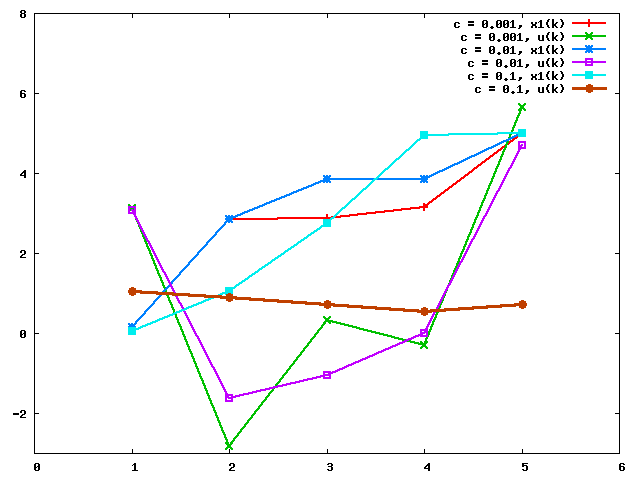
\includegraphics[width=\linewidth]{out}

From the graph, it appears that the $c = 0.01$ solution is the best compromise between accuracy and smoothness.

\newpage

\textbf{Regression Analysis:} \\

1. Chebychev Norm ($p = \infty$):

\begin{verbatim}
MIN = e;
B * 0 + a + e > 1;
B * 0 + a - e < 1;
B * 1.5 + a + e > 1.8;
B * 1.5 + a - e < 1.8;
B * 2.5 + a + e > 1.3;
B * 2.5 + a - e < 1.3;
B * 4.3 + a + e > 2.2;
B * 4.3 + a - e < 2.2;
B * 5.9 + a + e > 3.1;
B * 5.9 + a - e < 3.1;
B * 7.5 + a + e > 3.3;
B * 7.5 + a - e < 3.3;
B * 9.4 + a + e > 2.8;
B * 9.4 + a - e < 2.8;
\end{verbatim}

Results:

\begin{verbatim}
                       Variable           Value        Reduced Cost
                              E       0.5304348            0.000000
                              B       0.2173913            0.000000
                              A        1.286957            0.000000
\end{verbatim}

Minimum Absolute Value ($p = 1$):

\begin{verbatim}
MIN = e1p + e1m + e2p + e2m + e3p + e3m + e4p + e4m + e5p + e5m + e6p + e6m + e7p + e7m;
B * 0 + a + e1p - e1m = 1;
B * 1.5 + a + e2p - e2m = 1.8;
B * 2.5 + a + e3p - e3m = 1.3;
B * 4.3 + a + e4p - e4m = 2.2;
B * 5.9 + a + e5p - e5m = 3.1;
B * 7.5 + a + e6p - e6m = 3.3;
B * 9.4 + a + e7p - e7m = 2.8;
\end{verbatim}

Results:

\begin{verbatim}
                       Variable           Value        Reduced Cost
                            E1P        0.000000            1.302326
                            E1M        0.000000           0.6976744
                            E2P       0.3813953            0.000000
                            E2M        0.000000            2.000000
                            E3P        0.000000            2.000000
                            E3M       0.3976744            0.000000
                            E4P        0.000000            1.697674
                            E4M        0.000000           0.3023256
                            E5P       0.4534884            0.000000
                            E5M        0.000000            2.000000
                            E6P       0.2069767            0.000000
                            E6M        0.000000            2.000000
                            E7P        0.000000            2.000000
                            E7M       0.8232558            0.000000
                              B       0.2790698            0.000000
                              A        1.000000            0.000000
\end{verbatim}

For Least-Squares Analysis, after setting up the problem using the LINEST function, I get results: $y = 0.2331 x + 1.1787$. Data graph:

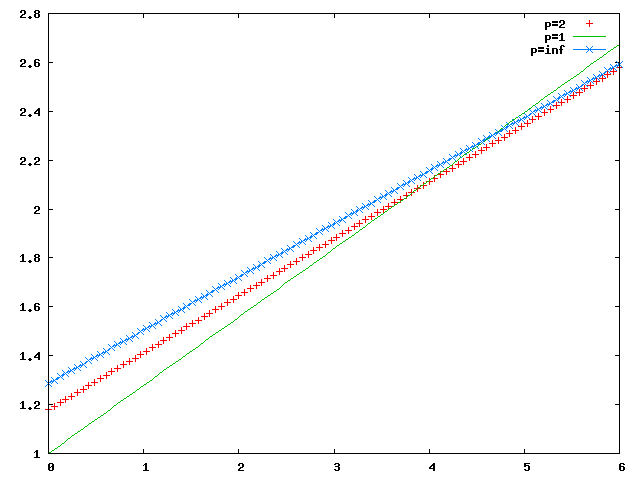
\includegraphics[width=\linewidth]{out1.png}

2. All reduced costs are $> 0$, so solutions are unique.

\end{document}